
\section{Objetivo}
\noindent Que el estudiante trabaje con un robot programable de tal forma que comprenda las funciones de distintos tipos de sensores y motores.

\section{Introducci\'on}

Se trabajará con Lego Mindstorms ya que es una plataforma fácil de usar y no es necesario tener conocimientos de circuitos digitales ni analógicos para la construcción del robot.

\subsection{¿Que es Lego Mindstorms?}

Lego Mindstorms es un paquete de software y hardware que permite crear robots programables, modulares y personalizables. Son caracterizados por contener una computadora central y módulos como: motores, actuadores, sensores de luz, de color, de presión, infrarrojos, etc. Y, como son Lego, se puede tener muchas configuraciones gracias a sus piezas intercambiables y construibles.


Ahora, para la práctica necesitaremos algunas cosas extras, ya que se utilizará el lenguaje de programación \classname{Python}, en lugar de usar la aplicación de diseño propia de Mindstorms. Se supondrá que se trabaja en Linux.

\subsection{Instalando ev3dev}

ev3dev es una distribución de Linux basada en Debian, lo cual permite tener una mayor disponibilidad de lenguajes y bibliotecas. La única desventaja es que sólo es compatible con la versión EV3 de Lego Mindstorms.

\noindent Se necesitará:

\begin{enumerate}
  \item El bloque programable de Mindstorms.
  \item Una memoria microSD con capacidad menor o igual a 32GB, preferentemente vacía ya que se borrarán todos los datos de esta.
  \item Una computadora con un adaptador para tarjetas microSD.
  \item Y una manera de comunicarse con el bloque programable, ya sea:
      \begin{itemize}
        \item Por un cable USB
        \item Por Wi-Fi usando un adaptador USB
        \item Por Ethernet usando un adaptador USB
        \item Por Bluetooth
      \end{itemize}
\end{enumerate}

\noindent Pueden obtener la imagen de ev3dev en: https://github.com/ev3dev/ev3dev/releases. Deben descargar la imagen que comienza con \quotes{ev3}, ya que las demás son para otros sistemas.

Una vez que tengan la imagen, procederemos a descomprimirla y copiarla a la memoria microSD:

\begin{enumerate}
  \item Abran una terminal y ejecuten el comando \classname{df} y guarden el resultado.
  \item Inserten la memoria y vuelven a ejecutar \classname{df} para obtener el nombre asignado por el sistema a su memoria.
  \item Desmonten la memoria, ejecutando \classname{sudo umount /dev/sdb1} (suponiendo que su memoria se encuentra en \classname{/dev/sdb1} ).
  \item Ahora, copiarán la imagen directamente a su memoria usando las aplicaciones \classname{dd} y \classname{xzcat}. Ejemplo: \classname{xzcat ~/Downloads/ev3dev-yyyy-mm-dd.img.xz | sudo dd bs=4M of=/dev/sdb}.
  \item Y por último, en cuanto termine la ejecución del paso anterior (puede demorar algunos minutos, no se desesperen), faltaría ejecutar \classname{sync} para asegurarse de que todas las escrituras al disco terminen y podrán remover la memoria microSD de su computadora.
\end{enumerate}


Después de haber descomprimido y escrito la imagen a la memoria, basta con insertarla al bloque programable y encenderlo.


\subsection{Conectándose a internet}

Para lograr una conexión a internet (y poder acceder al bloque por medio de \classname{ssh}), pueden consultar http://www.ev3dev.org/docs/getting-started/ donde encontrarán guías para cada método: por USB, usando un adaptador inalámbrico, usando un adaptador Ethernet USB o por bluetooth.


\subsection{Instalando Python, virtualenv y bibliotecas extras}

\subsubsection{¿Qué es virtualenv?}

Virtualenv es una aplicación que facilita hacer proyectos con Python, ya que crea un ambiente virtual en el que pueden utilizar una versión de Python específica, junto con \textit{add-ons} para esa versión, sin tener que utilizar esa misma versión globalmente. Léase: crea un contenedor con Python independiente.

\subsubsection{Instalación}
Una vez establecida una conexión por \classname{ssh} al bloque programable, basta ejecutar lo siguiente:

\begin{enumerate}
  \item \classname{apt-get update}
  \item \classname{apt-get install virtualenv virtualenvwrapper python-setuptools}\\ \classname{python-smbus python-pil}
  \item \classname{source /etc/bash\_completion.d/virtualenvwrapper}
  \item \classname{mkvirtualenv \{nombre del contenedor\} --python=/usr/bin/python2.7}\\ \classname{--system-site-packages}
  \item \classname{workon \{nombre del contenedor\}}
  \item \classname{easy\_install -U python-ev3}
\end{enumerate}

Con esto hecho, ya podrán acceder a los motores y sensores del EV3 desde Python, importando la biblioteca \classname{ev3}.\par

Para poder ejecutar su aplicación, pueden desarrollarla directamente desde el bloque programable usando \classname{vi} o \classname{nano}, pero se recomienda generar el archivo aparte y después copiarlo al bloque utilizando el comando \classname{scp}. Por ejemplo:

Suponemos que tenemos un archivo llamado \classname{seguidor\_de\_linea.py}, entonces ejecutamos:

\begin{itemize}
 \item \classname{scp seguidor\_de\_linea root@[dir\_ip\_bloque]:/home/robot}
\end{itemize}

Con esto, usando \classname{ssh}, nos dirigimos a la carpeta raíz del usuario y ejecutamos:

\begin{itemize}
 \item \classname{python seguidor\_de\_linea.py}
\end{itemize}

\section{Desarrollo e implementación}

Su práctica consiste en crear un robot seguidor de línea y un algoritmo para éste.

\subsection{Robot}

Pueden utilizar el sensor de color (para identificar la línea) y los distintos motores que tienen a su disposición. El diseño del robot es libre, un ejemplo de cómo montar los motores y sensor lo pueden ver en la figura~\ref{fig:P10robot}.

\subsection{Algoritmo}

Aquí tienen un ejemplo que utiliza dos motores (también lo pueden encontrar en el apéndice~\ref{appe:lego}), ubicados en los costados del bloque programable, y el sensor de color para ubicarse. Cabe notar que este algoritmo es bastante sencillo, ustedes deberán mejorarlo para que su robot siga la línea lo más fluidamente posible.

\begin{minted}[mathescape,
               linenos,
               numbersep=5pt,
               gobble=2,
               frame=lines,
               framesep=2mm]{python}
  from ev3.ev3dev import Motor
  from ev3.lego import ColorSensor

  a = Motor(port=Motor.PORT.A) # Abre el motor en el puerto A
  b = Motor(port=Motor.PORT.D) # Abre el motor en el puerto D
  sense = ColorSensor() # Abre el sensor para leer los valores
                        # que obtiene

  def move():
      maxSpeed = 100
      black = 10
      white = 78
      speedA = 50
      speedB = 50
      midpoint = (white-black)/2 + black
      tolerance = 20
      last_error = 0

      while True:
          # Obtiene el valor de reflectividad de la superficie
          # que ve el sensor
          val = sense.reflect 
          error = midpoint - val
          print error, val

          if abs(error) < tolerance:
              speedA = maxSpeed - last_error/2
              speedB = maxSpeed - last_error/2
              last_error = error
          else:
              if error > 0:
                  speedB = speedB + error/2
                  speedA = speedA - error/2
                  last_error = error
              else:
                  error = abs(error)
                  speedB = speedB - error/2
                  speedA = speedA + error/2
                  last_error = error

          if speedA < 0: speedA = 0
          if speedA > maxSpeed: speedA = maxSpeed
          if speedB < 0: speedB = 0
          if speedB > maxSpeed: speedB = maxSpeed

          # Hace que el motor A gire a la velocidad especificada
          # indefinidamente
          a.run_forever(speedA) 
          # Hace que el motor B gire a la velocidad especificada
          # indefinidamente
          b.run_forever(speedB) 
\end{minted}

Lamentablemente no hay mucha documentación sobre este plug-in, pero siempre pueden consultar más ejemplos en: https://github.com/topikachu/python-ev3

\section{Requisitos y resultados}

Deben entregar un script o aplicación que resuelva el problema de seguir una línea negra u obscura en un fondo contrastante junto con imágenes de la construcción del robot. Su script deberá ser lo más eficiente posible y debe guiar al robot a una velocidad mayor que el ejemplo que aparece en la sección anterior.


\begin{figure}[H]
  \begin{subfigure}{.5\textwidth}
    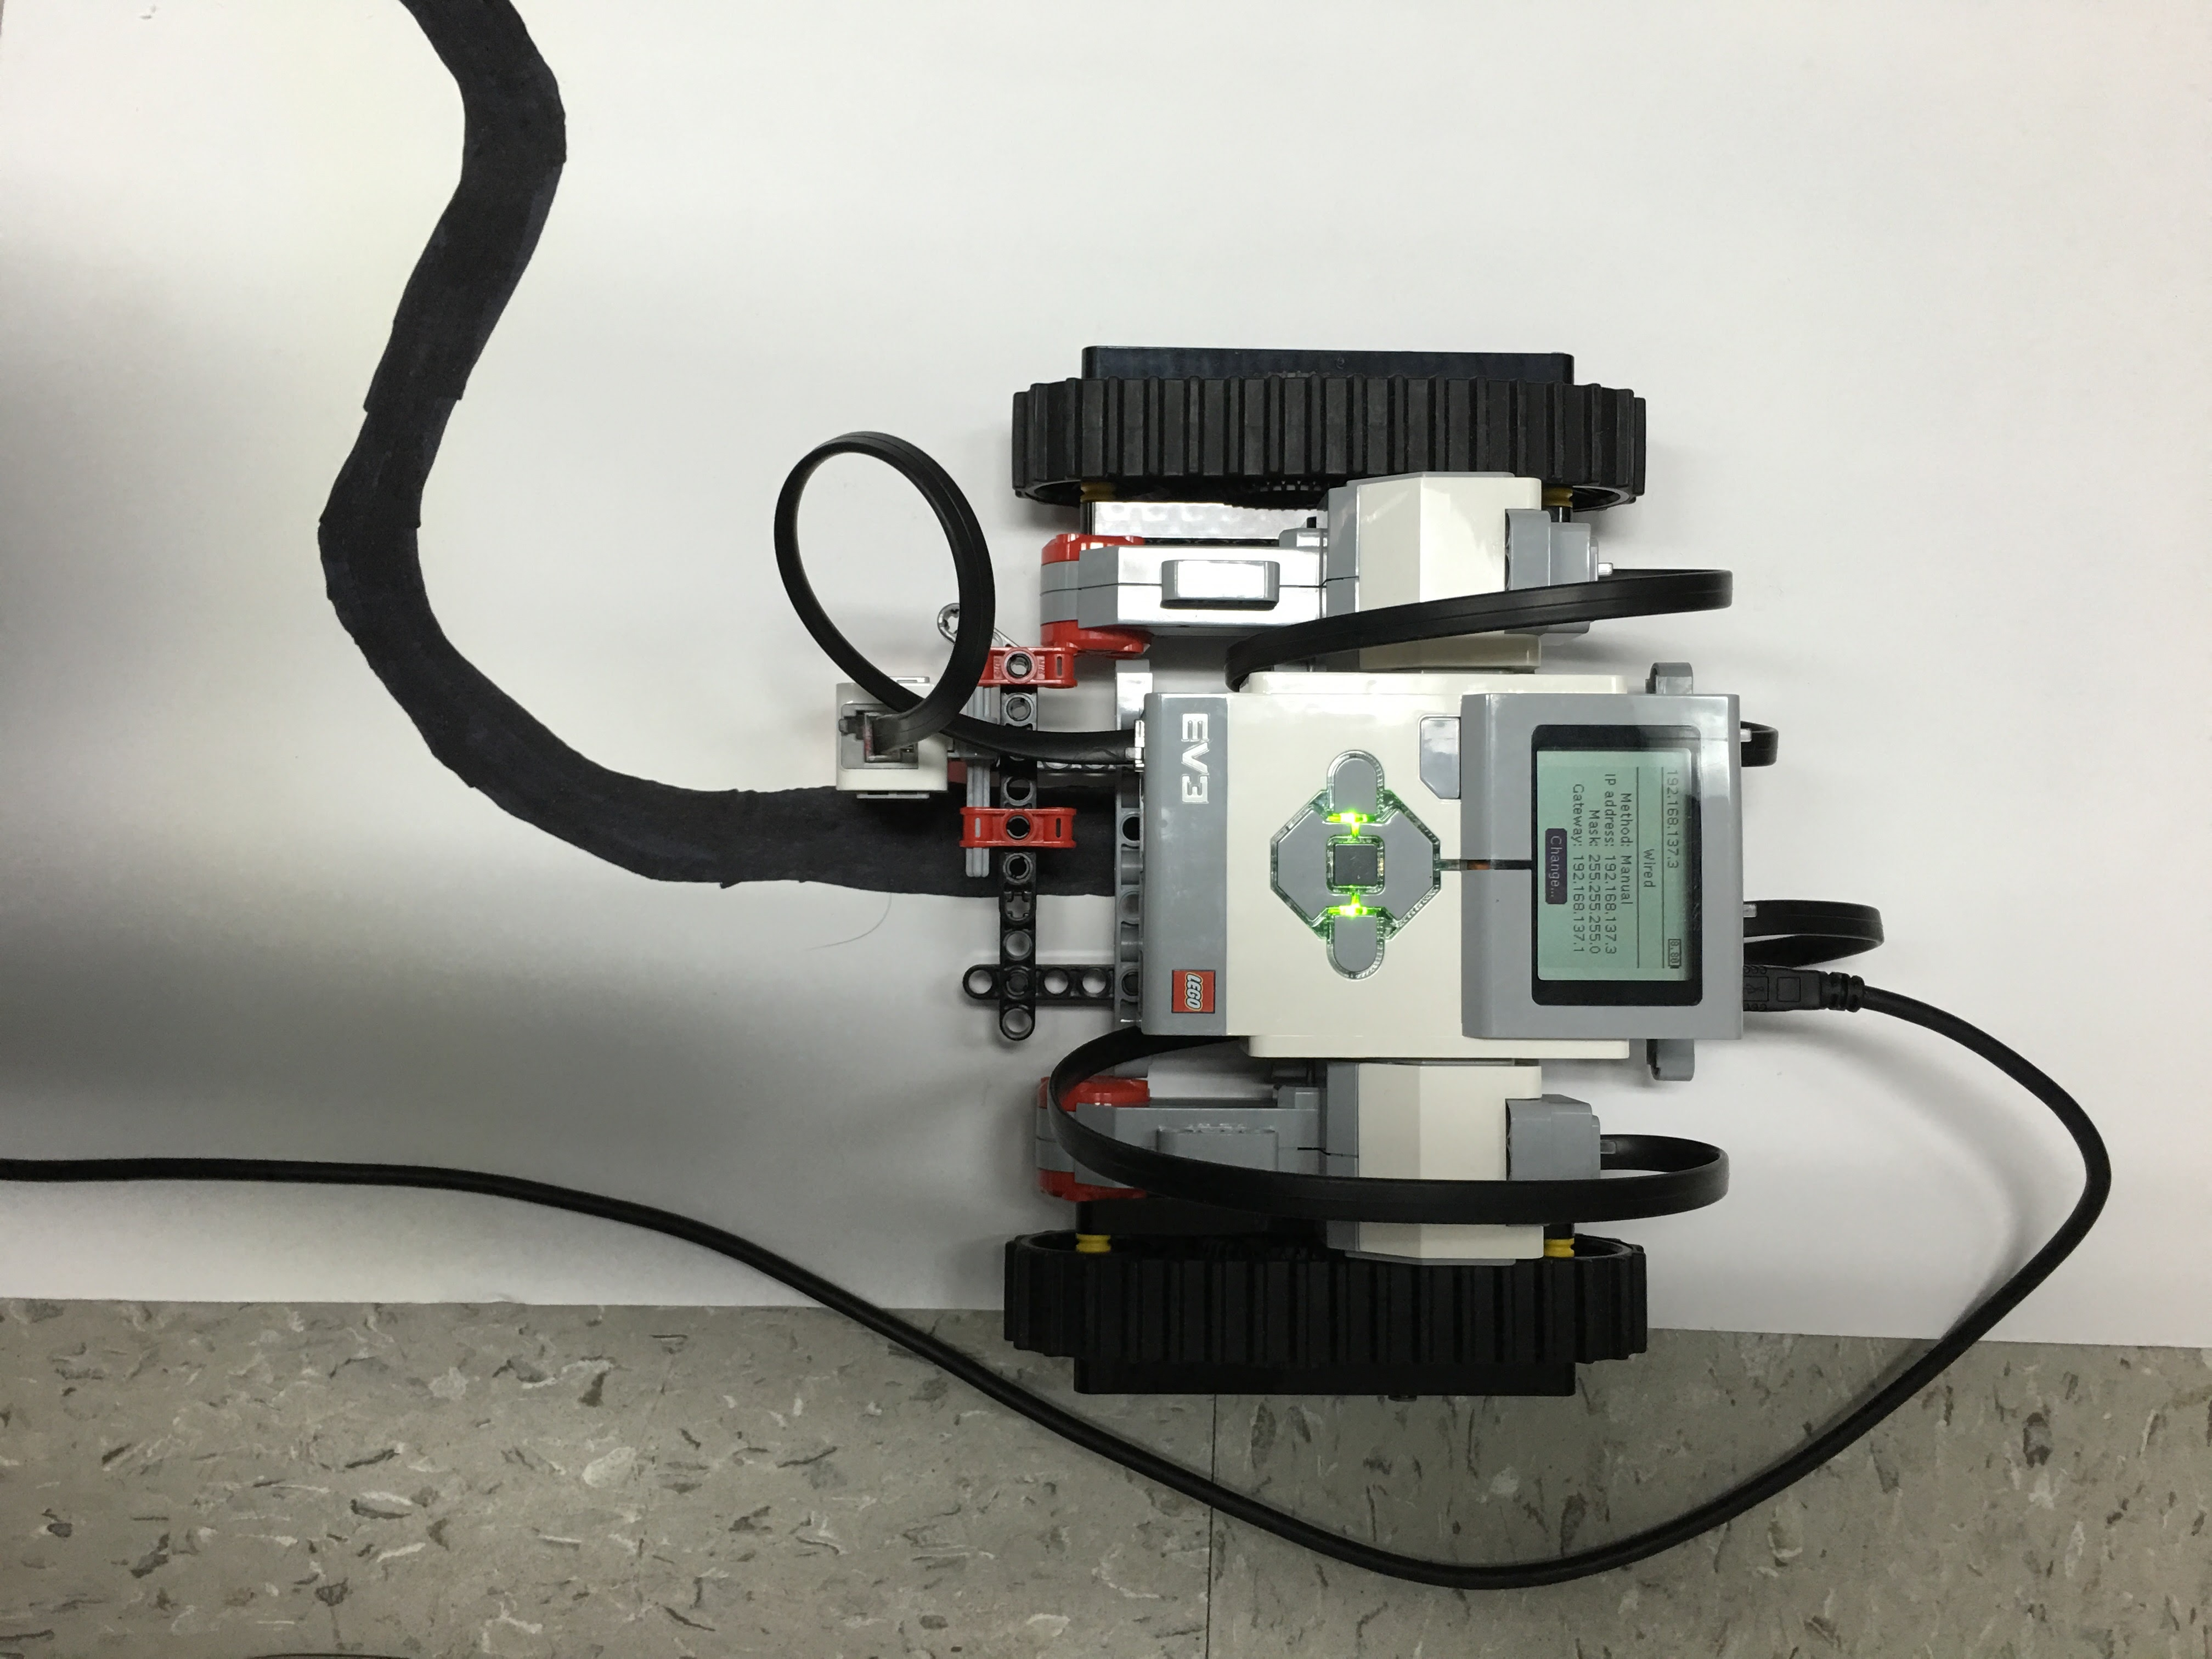
\includegraphics[scale=0.053]{legomindstorm/IMG_1892.JPG}
    % \includegraphics[width=.4\linewidth]{image1}
  \end{subfigure}
  \begin{subfigure}{.5\textwidth}
    % \includegraphics[width=.4\linewidth]{image1}
    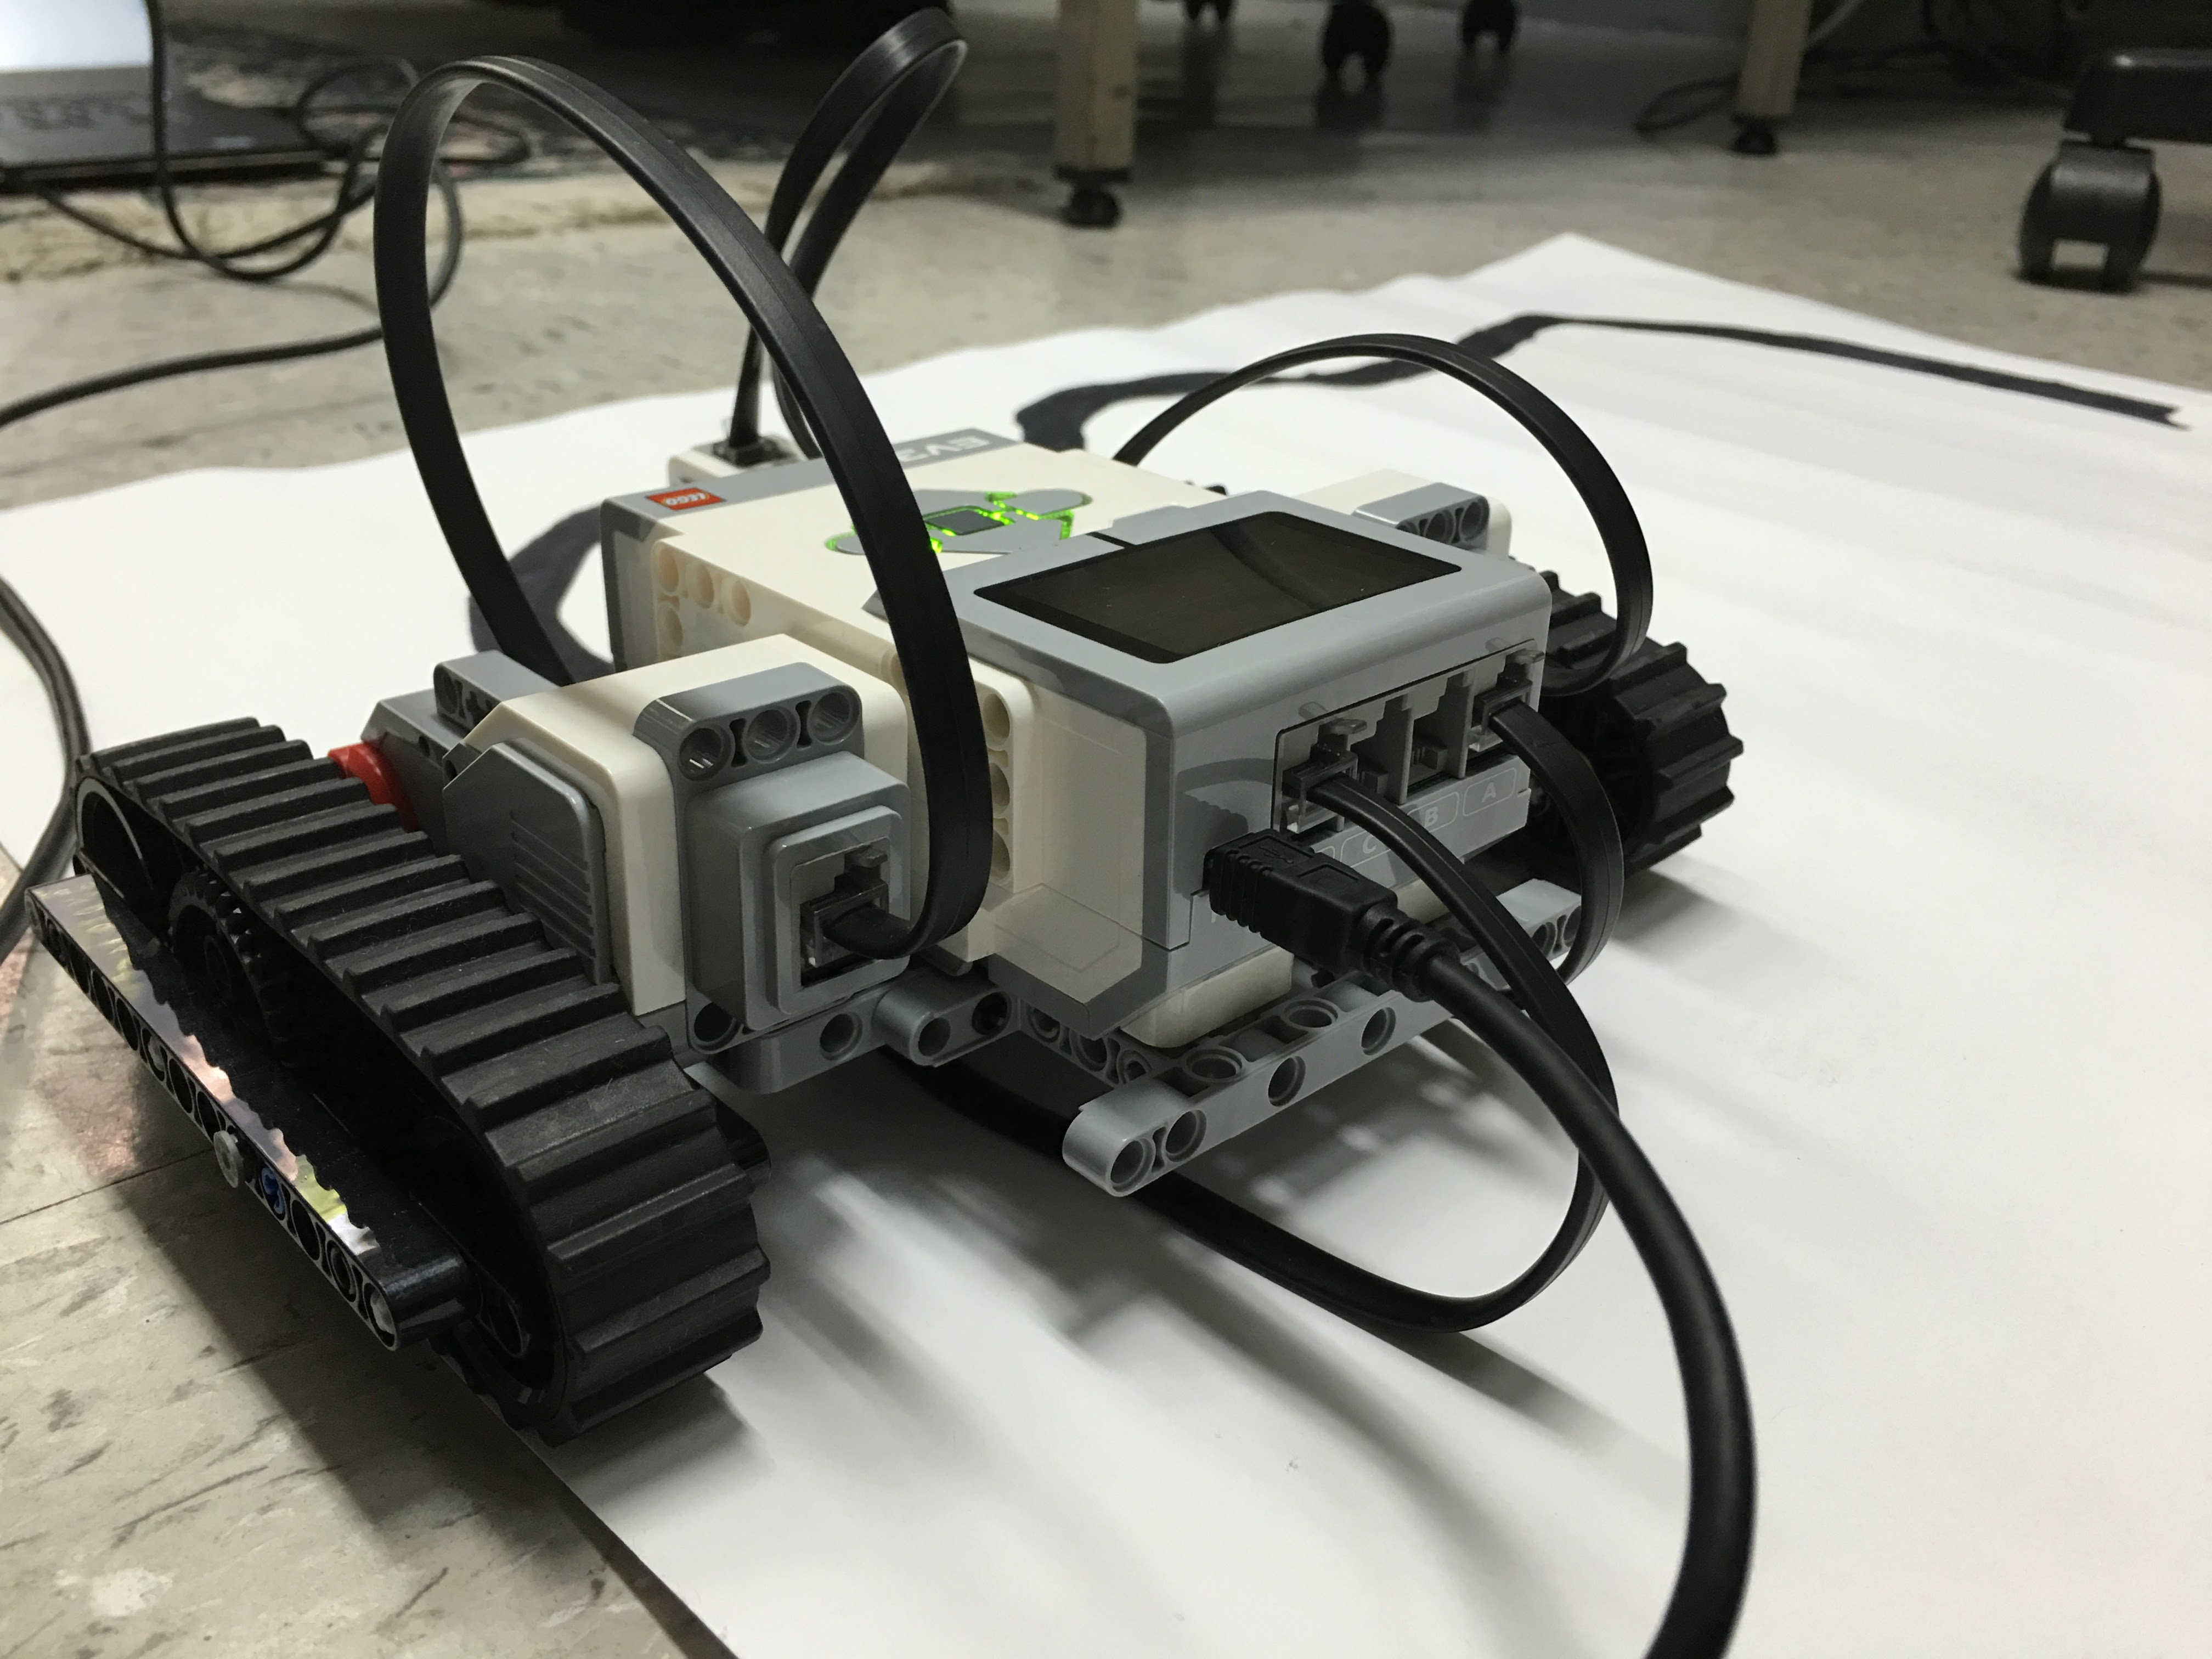
\includegraphics[scale=0.053]{legomindstorm/IMG_1895.JPG}
  \end{subfigure}
  \caption{Aquí se muestra una configuración ejemplo de robot seguidor de línea utilizando Lego Mindstroms.}
  \label{fig:P10robot}
\end{figure}

% \begin{thebibliography}{1}

  % \bibitem{notes} Michael Negnevitsky {\em Artificial Intelligence: A guide to Intelligent Systems}, 2005 :
  % Pearson Education Limited, Essex, England .

% \end{thebibliography}

